\documentclass[
 aip,
 jmp,
 amsmath,amssymb,
 reprint
]{revtex4-1}

\usepackage[utf8]{inputenc}
\usepackage[T1]{fontenc}
\usepackage[francais]{babel}
\usepackage{graphicx}
\usepackage{float}
\usepackage{listings}
\usepackage[colorlinks = true, 
            urlcolor = blue]{hyperref}
\usepackage{caption}
\usepackage{dcolumn}
\usepackage{bm}
\lstset{columns=flexible}
\lstset{keepspaces=false}
\begin{document}

\title{Comparatif des performances d'une application en fonction des paramètres de compilation utilisés et analyse des performances}

\author{Pierre \textsc{Tassel} sous la direction de Sid \textsc{Touati}}

\date{\today}

\begin{abstract}
L'utilisation d'outils tels que Gprof et la suite parallel Studio XE d'Intel\copyright \, nous permettent une analyse plus poussée des programmes et ouvrent la voie vers de possibles optimisations.
\end{abstract}

\maketitle

\begin{quotation}
Dans le but de nous familiariser avec les outils d'analyse de performances d'Intel et du projet GNU, nous allons analyser un algorithme de type MinMax avec coupe Alpha Bêta sur l'une des variantes du jeu Awale avec 6 cases par joueur écrit en C++. Le but étant de déterminer la meilleure façon de compiler ce programme (compilateur et options à utiliser), d'analyser ce programme pour déterminer ce qui ralentit son exécutions ainsi que de tenter de l'optimiser par différents moyens.
\end{quotation}

\section{Introduction}
\subsection{Programme à analyser}
Le code à analyser étant dépendant de Windows (import de la bibliothèque windows.h), il faut le réécrire pour permettre de le rendre non dépendant d'un os en particulier. Cette bibliothèque est utilisé pour les compteurs de temps, il est donc facile de réécrire le programme afin qu'il soit indépendant de l'OS en utilisant les fonctions de la librairie standard.\\
Ce programme utilise un algorithme de MinMax avec coupes alpha bêta pour choisir le coup à jouer, le principe d'un algorithme MinMax est de parcourir jusqu'à une certaine profondeur l'arbre des coups possibles à un état donné du jeux et d'attribuer un score à chaque coup possible, il choisira ensuite le coup qui lui est le plus favorable en partant du principe que l'adversaire choisira les meilleurs coups. Les coupes alpha bêta sont juste une technique permettant d'aller plus profondément dans l'arbre des coups possibles en éliminant certains mauvais coups et évitant ainsi beaucoup d'explorations inutiles.

\subsection{Environnement d'analyse}
\subsubsection{Logiciel}
Afin d'analyser le programme efficacement, il faut aussi mettre en place un environnement propice à l'analyse des performances, pour cela nous utiliserons un système d'exploitation en CLI, avec le minimum de service possible installé. Nous utiliserons donc Arch Linux, basé sur le noyau Linux 4.14.13-1 cette distribution possède le minimum d'applications et de services possible installé.\\

\subsubsection{Matériel}
Notre environnement expérimental est un ordinateur portable utilisant un processeur Intel I7-4710HQ, 8Go de RAM en DDR3, un SSD et le processeurs scaling a été désactivé dans le BIOS, cela permet de faire tourner le processeur à vitesse constante et ainsi ne faussant pas les résultats.

\section{Analyse des options de compilations optimaux}
\subsection{Démarche expérimentale}
Il faut tout d'abord modifier le programme pour qu'il n'affiche en sortie uniquement le temps d'exécution de la partie et non plus les informations utiles aux joueurs.\\
Ensuite, il faut obtenir un ensemble de données. Sachant que le programme est déterministe (pas de modification de la profondeur en fonction du temps, ni de random) les mêmes entrées (coups joués par nous) produiront les mêmes sorties (coups joués par le logiciel). Il nous suffit donc de posséder une liste de coup à envoyer sur la sortie standard des différentes versions du programme (obtenue à partir des différentes options de compilations utilisé) et nous obtiendrons le temps d'exécution de chacun.\\
Afin d'obtenir les entrées du programme, nous avons fait tourner deux instance du programme, l'un jouant le joueur 1, le second jouant le joueur 2 et nous avons noté les coups joués par chacun.\\
A la fin de l'obtention de ces différents coups, nous pouvons déduire que le temps d'exécution sera à analyser en seconde, vu que la partie est plutôt longue.\\
Nous créerons ensuite une script exécutant les différentes compilations et exécuteras les programmes 20 fois chacun pour chaque partie (une fois où le programme commence, une fois où le joueur commence). Cela permettra de déterminer quel est le meilleur compilateur et avec quels options.\\
Ce script étant lent à être totalement exécuter (il y a 480 exécutions différentes au total) nous l'exécuterons au travers de la commande nohup afin d'éviter toute interruption possible.\\

\subsection{Résultats}
En regardant les temps d'exécutions configuration par configuration nous observons que les temps d'exécutions sont plutôt stables. Nous choisissons donc d'afficher les résultats sous forme de barres représentant la médiane des temps d'exécutions de chaque configurations.\\

\begin{figure}[H]
  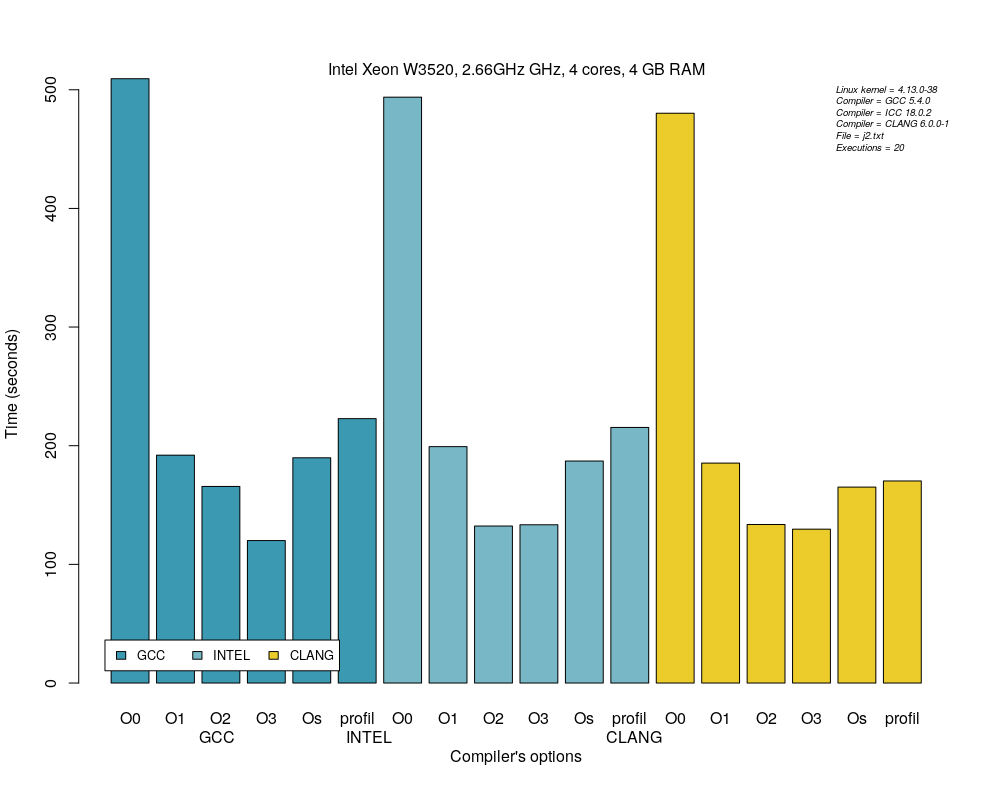
\includegraphics[width=\linewidth, keepaspectratio=true]{GCCvsICCvsCLANG_j2.png}
  \caption{Temps d'exécutions quand le programme commence\label{Fig:temps_exec_j2}}
  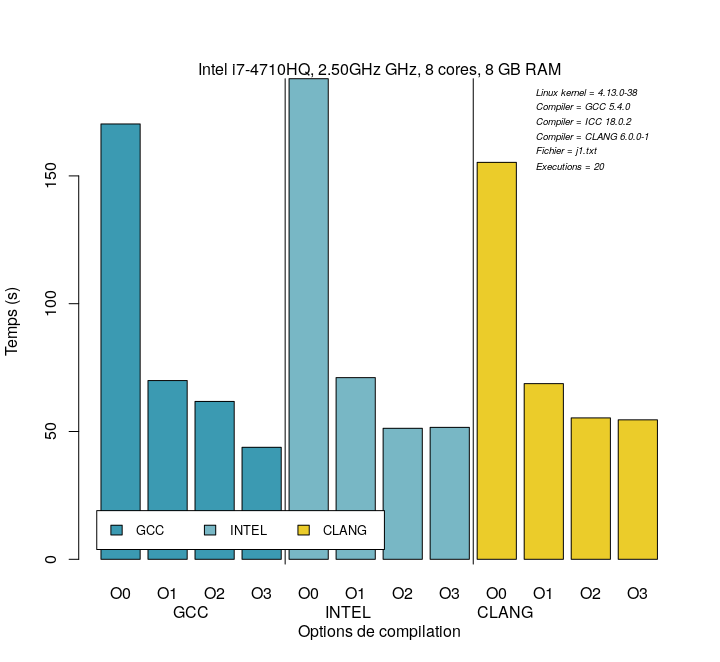
\includegraphics[width=\linewidth, keepaspectratio=true]{GCCvsICCvsCLANG_j1.png}
  \caption{Temps d'exécutions quand le joueur commence\label{Fig:temps_exec_j1}}
\end{figure}

On remarque que le fait que le joueur commence ou non n'a pas d'influence sur le choix du compilateur, on pourra donc ce concentrer sur l'analyse des temps d'exécutions quand le programme commence.\\
On remarque aussi que GCC avec l'option O3 activé est le meilleur compilateur pour ce programme.\\
Pour GCC et Intel, chaque niveau d'optimisation réduit grandement le temps d'exécution, il y a un rapport de 4 entre la compilation sans optimisation (O0) et la compilation avec le plus d'optimisations (O3). Cette différence est légèrement inférieure avec Clang car la version sans optimisation (O0) est plus rapide que celle des autres compilateurs, mais elle reste importante (rapport de 3).\\
Une chose étonnante est que la version O2 d'Intel est légèrement plus rapide que la version O3.\\

\subsubsection{Taille des exécutables}
\begin{figure}[H]
  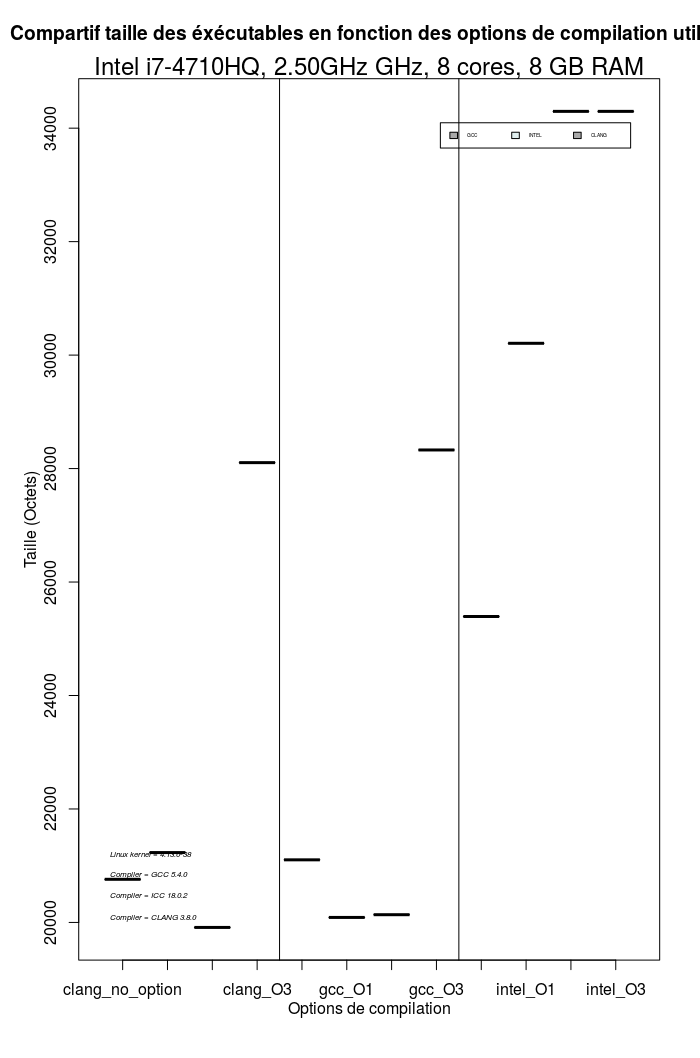
\includegraphics[width=\linewidth, keepaspectratio=true]{sizes.png}
  \caption{Comparatif des tailles d'exécutables produits par les diverses méthodes de compilations\label{Fig:taille_executables_seq}}
\end{figure}

La aussi GCC avec l'option O3 semble être la aussi la meilleure option pour ce programme.

\section{Profilage du code}

Il existe deux grands logiciels pour analyser les performances d'un programme et les fonctions chaudes, GProf qui est un logiciel libre et vTune qui est un logiciel propriétaire appartenant appartenant à Intel. Nous allons utiliser ces deux logiciels, afin de trouver des possibilités d'optimisation de code.

\subsection{Gprof}

\begin{lstlisting}[
    basicstyle=\tiny, %or \small or \footnotesize etc.
]
Each sample counts as 0.01 seconds.                 
 time   seconds   seconds    calls   s/call   s/call  name    
 48.83    167.72   167.72 5172852992     0.00     0.00  jouer_coup(Next*, Pos*, Pos*, int, int)
 18.25    230.39    62.67 3262157329     0.00     0.00  copier(Pos*, Pos*)
 17.22    289.56    59.16 3262157262     0.00     0.00  est_affame(Pos*, int)
  8.79    319.75    30.20 1457826958     0.00     0.00  calculer_coup(Next*, Pos*, int, int, int, int, bool)
  5.31    337.98    18.23 3252245939     0.00     0.00  valeur_minimaxAB(Next*, Pos*, int, int, int, int, bool)
  0.87    340.99     3.00 1775297034     0.00     0.00  evaluer(Pos*)
  0.52    342.77     1.79       67     0.03     0.03  test_fin(Pos*)
  0.16    343.34     0.57                             print_position_ordi_haut(Pos*)
  0.09    343.65     0.31       33     0.01    10.34  decisionAB(Next*, Pos*, int, bool)
  0.01    343.70     0.05                             decision(Next*, Pos*, int)
  0.00    343.71     0.01        1     0.01     0.01  _GLOBAL__sub_I__Z13init_positionP3Pos
  0.00    343.71     0.00       67     0.00     0.00  print_position_ordi_bas_inv(Pos*)
  0.00    343.71     0.00        1     0.00     0.00  position_debut(Pos*)
  0.00    343.71     0.00        1     0.00     0.00  __static_initialization_and_destruction_0(int, int)
\end{lstlisting}

Il nous apprend que la fonction la plus utilisé est jouer\_coup, et ce très largement. On note aussi que la fonction decisionAB est moins souvent appelé mais chaque appel est d'une plus longue durée.\\
Ce sont donc les deux fonctions qu'il faut tenter d'optimiser en priorité pour améliorer les performances d'après Gprof.\\

\subsection{Intel vTune}
\begin{figure}[H]
  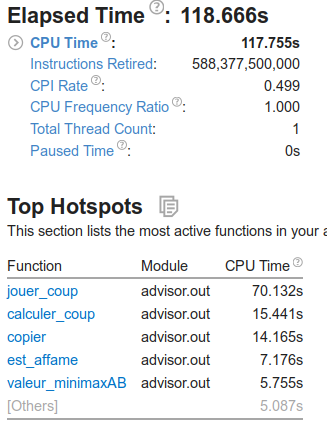
\includegraphics[width=\linewidth, keepaspectratio=true]{vtune.png}
  \caption{Profilage du code avec vTune\label{Fig:vTune_sequentiel_cpu}}
\end{figure}

Comme Gprof, vTune nous indique que c'est la fonction jouer\_coup qui a pris le plus de temps à calculer. Cependant, il place calculer\_coup second contrairement a GProf.\\
Il nous apprend aussi que seul un processeur est utilisé sur les 8 disponibles. Il y a donc un manque de parallélisme, ce qui ouvre une première voie vers une possible optimisation.\\
Nous pouvons aussi utiliser ce logiciel pour analyser les accès mémoire.\\

\begin{figure}[H]
  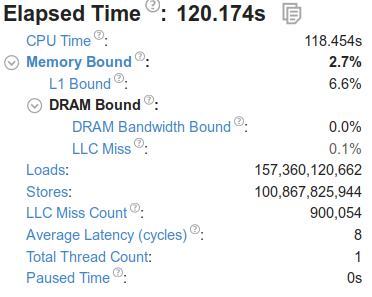
\includegraphics[width=\linewidth, keepaspectratio=true]{memory_vtune.png}
  \caption{Profilage des accès mémoire\label{Fig:vTune_sequentiel_mem}}
\end{figure}

On remarque très clairement que le programme n'est pas "Memory Bottleneck" mais "CPU Bottleneck" (le CPU est le facteur limitant de cette application).\\
Car il y a très peu d'erreurs de cache et les accès mémoire sont petits.

\section{Ajout de parallélisme}

Comme ce programme est CPU Bottleneck et qu'il n'y a qu'un seul processeur utilisé, l'ajout de parallélisme semble être une possibilité d'optimisation.

\subsection{Approche naïve}
On a ajouté du parallélisme un peu partout où il n'y a pas de dépendance de données en utilisant la librairie OpenMP.\\
Malheureusement il a été impossible de rajouter du parallélisme de contrôle, mais seulement du parallélisme de donnée, on peut d'or et déjà s'attendre à ce que le parallélisme soit peux pertinent vu la faible taille des données et la simplicité des actions effectués dans chacune des itérations des boucles parallélisées.\\
Ensuite, nous réitérons ce que nous avons fait pour la version sans parallélisme en utilisant chaque compilateur avec l'option O3 activé mais, en faisant varier le nombre de processeurs pour déterminer le nombre optimal de processeur à utiliser.\\

\subsubsection{Résultats}\mbox{}\\

Nous représentons les résultats sous forme de \href{https://en.wikipedia.org/wiki/Violin_plot}{Violin Plot} nous permettants de représenter à la fois les écarts types et la fonction de densité.

\begin{figure}[H]
  \caption{Parallélisme naïf avec un processeur}
  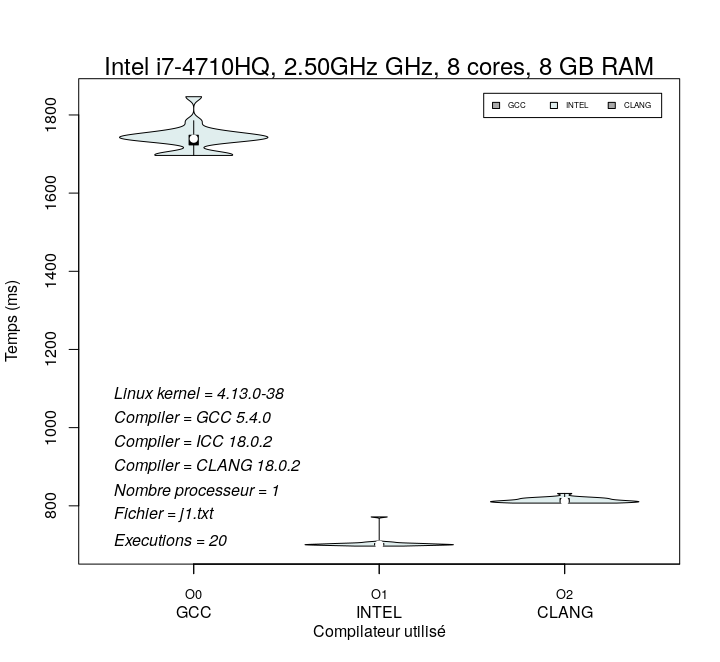
\includegraphics[width=\linewidth, keepaspectratio=true]{naif_1.png}
\end{figure}

\begin{figure}[H]
  \caption{Parallélisme naïf avec deux processeurs}
  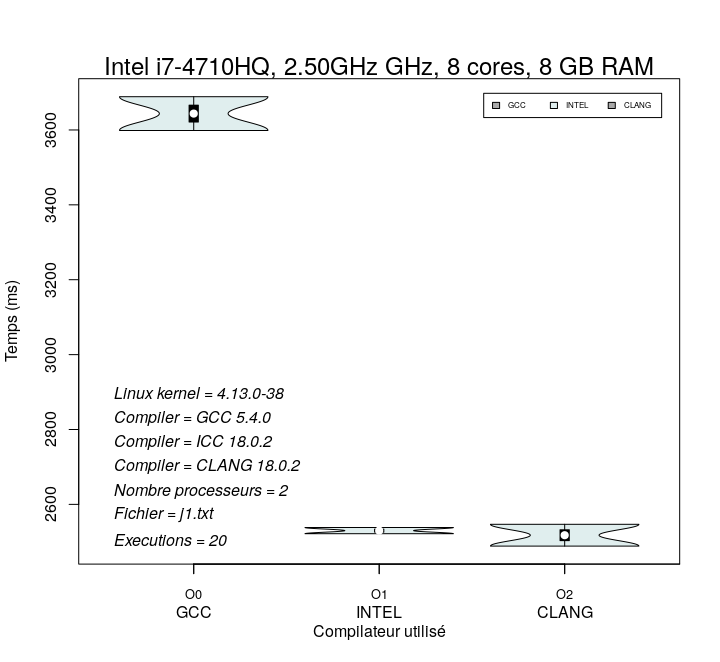
\includegraphics[width=\linewidth, keepaspectratio=true]{naif_2.png}
\end{figure}

\begin{figure}[H]
  \caption{Parallélisme naïf avec trois processeur}
  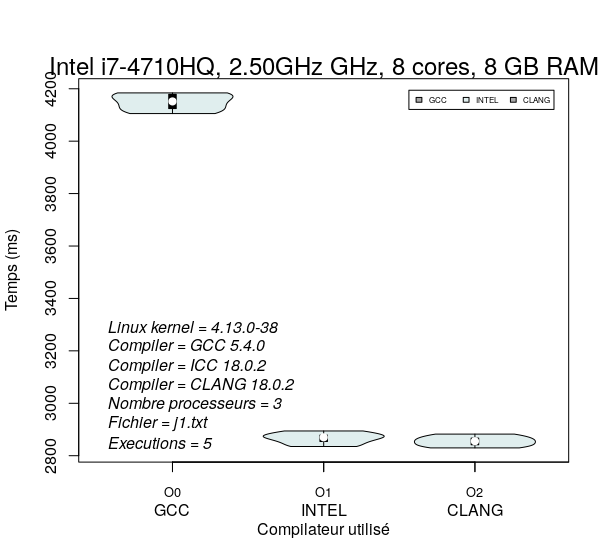
\includegraphics[width=\linewidth, keepaspectratio=true]{naif_3.png}
\end{figure}

\begin{figure}[H]
  \caption{Parallélisme naïf avec quatre processeurs}
  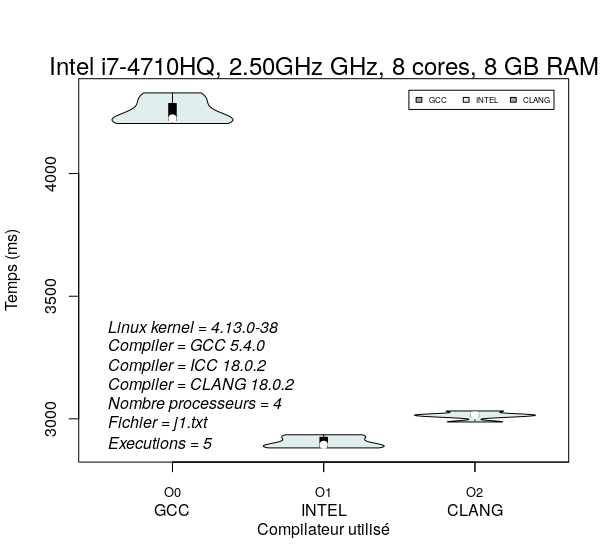
\includegraphics[width=\linewidth, keepaspectratio=true]{naif_4.png}
\end{figure}

\begin{figure}[H]
  \caption{Parallélisme naïf avec cinq processeur}
  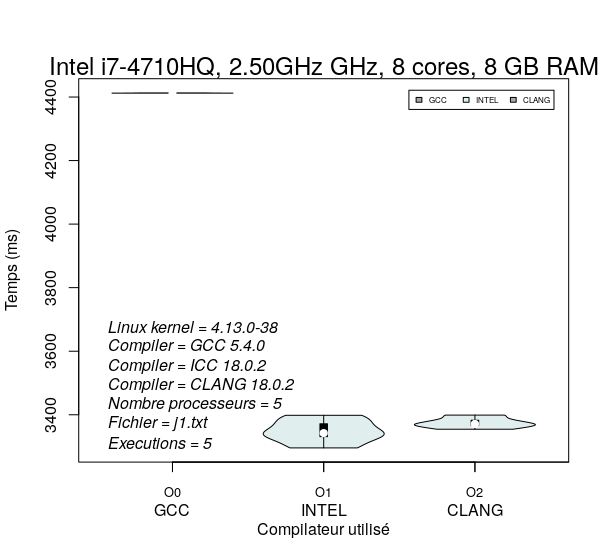
\includegraphics[width=\linewidth, keepaspectratio=true]{naif_5.png}
\end{figure}

\begin{figure}[H]
  \caption{Parallélisme naïf avec six processeurs}
  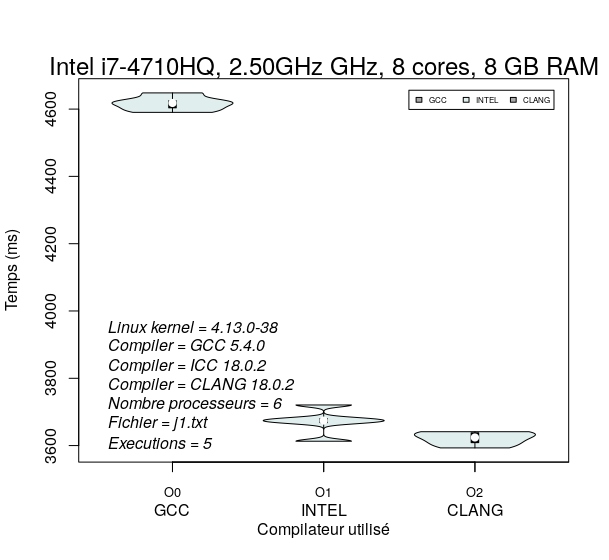
\includegraphics[width=\linewidth, keepaspectratio=true]{naif_6.png}
\end{figure}

\begin{figure}[H]
  \caption{Parallélisme naïf avec sept processeur}
  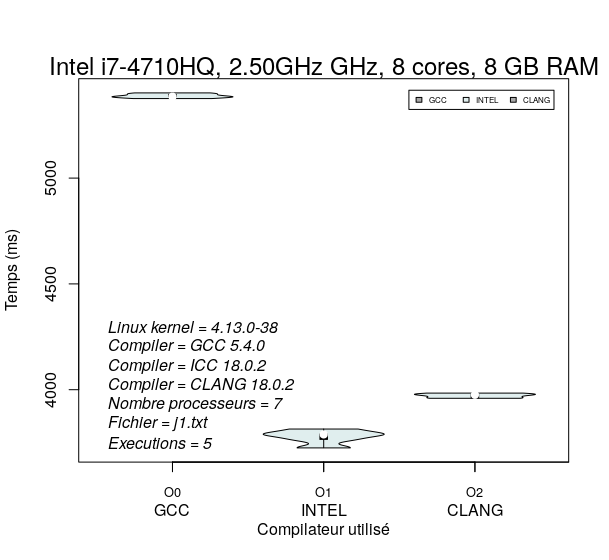
\includegraphics[width=\linewidth, keepaspectratio=true]{naif_7.png}
\end{figure}

\begin{figure}[H]
  \caption{Parallélisme naïf avec huit processeurs}
  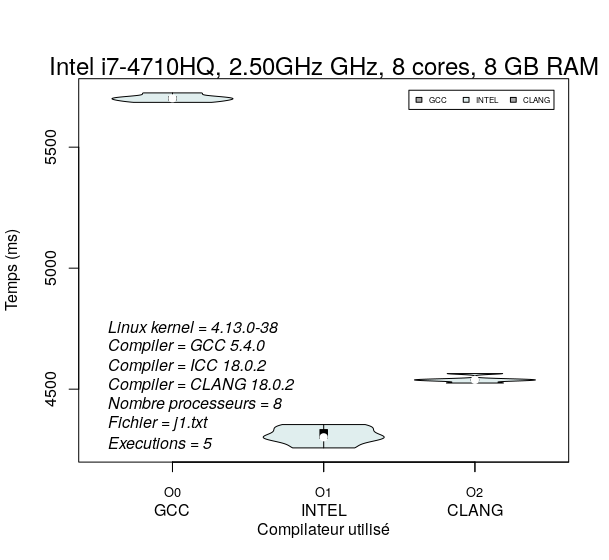
\includegraphics[width=\linewidth, keepaspectratio=true]{naif_8.png}
\end{figure}

Nous devons malheureusement réduire le nombre d'exécutions par configuration passant de 20 à 5, car le temps d'exécutions est extrêmement lent.\\
On remarque ici que Clang et Intel sont côte à côte niveau performance et qu'ici GCC pourtant le plus rapide sur le code séquentiel est le plus lent avec la version parallèle.\\
On remarque aussi que le temps d'exécutions c'est nettement dégradé quelque soit le compilateur utilisé et qu'il se détériore de plus en plus quand on ajoute un plus grand nombre de processeurs. Cela est du à deux facteurs : 
\begin{enumerate}
\item Le phénomène de False Sharing, les différents processeurs doivent assurer la cohérence des caches, à chaque fois qu'un processeur modifie une donnée, il invalide le cache d'un autre processeur s'il modifie la même ligne cache. Ce qui explique pourquoi augmenter le nombre de threads n'améliore pas les performances du programme, mais au contraire le ralentit encore plus.
\item OpenMP casse les optimisations du compilateur en ajoutant du code qui va aveugler le compilateur. Cela explique pourquoi les performances sont nettement inférieure entre le code séquentiel et le code avec un seul thread.
\end{enumerate}

\begin{figure}[H]
  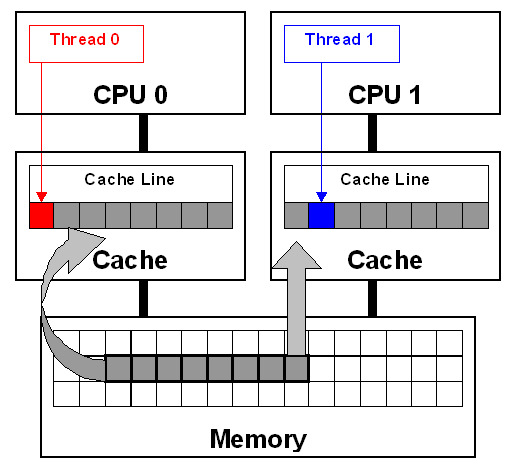
\includegraphics[width=\linewidth, keepaspectratio=true]{false_sharing.jpg}
  \centering
  \caption{Mecanisme de False Sharing\label{Fig:scatter_compact}}{\href{https://software.intel.com/en-us/articles/avoiding-and-identifying-false-sharing-among-threads}{Source : Documentation Intel}
}
\end{figure}

\subsection{Tentative d'amélioration des performances du code parallel en modifiant le placement des threads}\mbox{}\\

Un facteur qui peut être important dans les performances des codes parallèles est la manière dont sont placés les threads, cette méthode de placement de thread est appelé le "thread affinity".

\begin{figure}[H]
  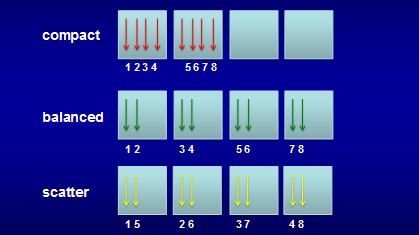
\includegraphics[width=\linewidth, keepaspectratio=true]{affinity.png}
  \centering
  \caption{Différentes méthode de placement de thread \label{Fig:affinity}}{\href{https://cvw.cac.cornell.edu/mic/affinity}{Cornell University}}
\end{figure}

Nous allons voir si modifier le placement des threads améliore ou non les performances parallèles en utilisant le compilateur d'Intel avec 8 threads car c'est l'un des compilateurs qui offrait les meilleurs performances parallèle et il a une gestion du placement des threads plus complète que Clang. Nous testerons deux méthodes de placement "Compact" et "Scatter" supporté par le compilateur Intel en utilisant la variable d'environnement \href{https://software.intel.com/en-us/node/522691}{KMP\_AFFINITY}.

\begin{figure}[H]
  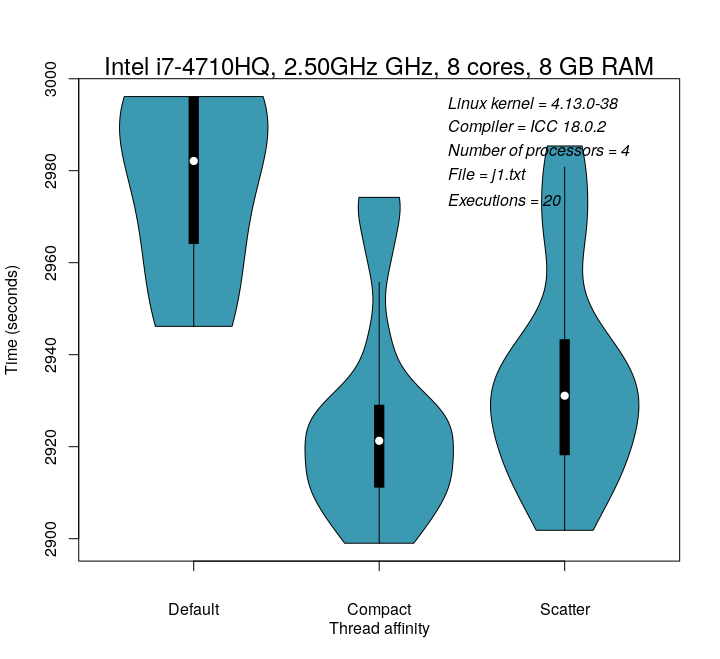
\includegraphics[width=\linewidth, keepaspectratio=true]{defaultVSscatterVScompact.png}
  \caption{Comparaison performances Scatter vs Compact\label{Fig:scatter_compact}}
\end{figure}

On remarque que les performances se sont bien améliorées par rapport au mode de placement par défaut (celle de l'OS lui même). Les performances de Compact et Scatter sont à peux près équivalentes pour ce programme ci dans cette configuration.

\subsection{Intel Advisor}
Advisor est un autre logiciel de la suite parallel studio qui, en plus de nous informer sur les fonctions chaudes du programme, nous donne des indications sur comment optimiser le code.\\
Nous avons vu que l'ajout naïf de parallélisme était défavorable aux performances du programme, nous allons ici tenter d'ajouter du parallélisme de manière plus intelligent à l'aide des outils de la suite Intel Parallel Studio XE.\\

\begin{figure}[H]
  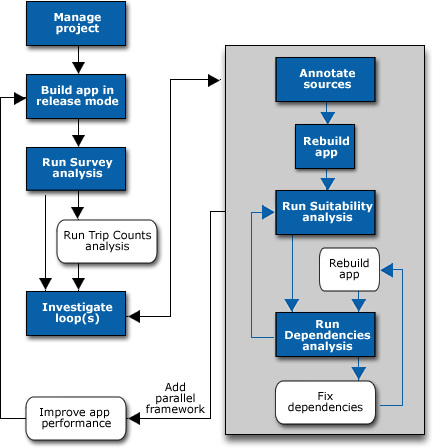
\includegraphics[width=\linewidth, keepaspectratio=true]{Intel.jpg}
  \caption{Processus itératif d'amélioration des performances\label{Fig:intel_processes}}
\end{figure}

\paragraph{Fonctions chaudes et optimisations}\mbox{}\\
D'abord, nous analysons le programme en cherchant les fonctions chaudes et les différents problèmes pouvant réduire les performances du programme.\\

\begin{figure}[H]
  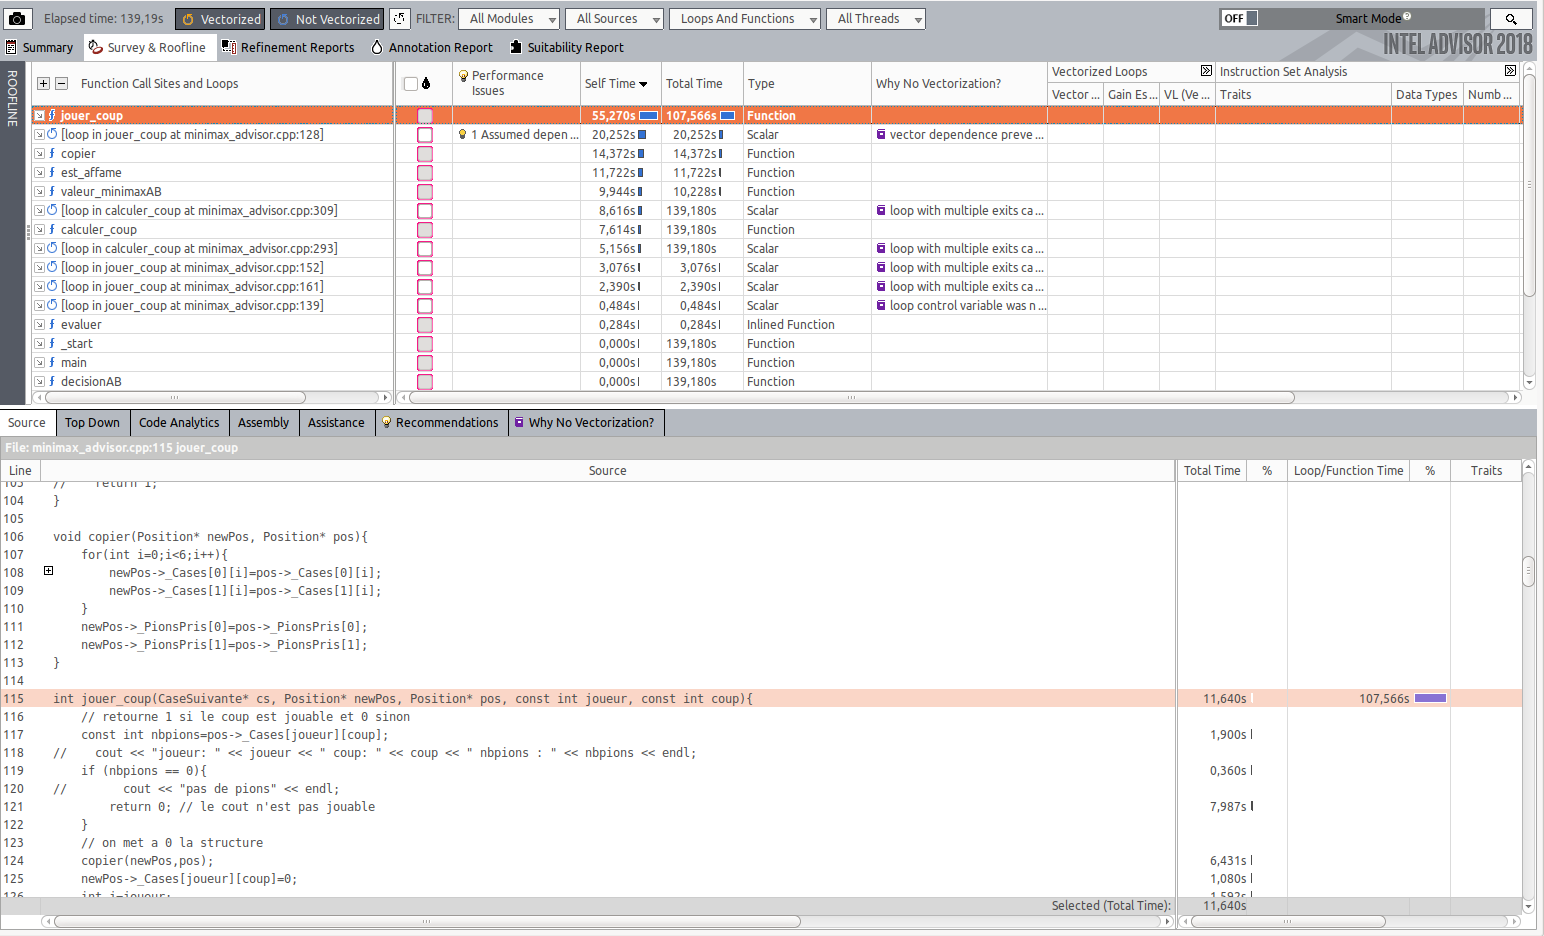
\includegraphics[width=\linewidth, keepaspectratio=true]{survey.png}
  \caption{Résultat d'Advisor "Survey"\label{Fig:advisor_survey}}
\end{figure}

Contrairement à vTune, Advisor donne aussi des indications sur ce qui nuit aux performances du programme. Par exemple nous avons ici une dépendance de donnée qui empêche la vectorisation. Malheureusement nous ne pouvons pas la supprimer, car c'est une dépendance Read after Write (dite "true dependancy").\\

\subsubsection{Test opportunité de parallélisme}\mbox{}\\
Il faut donc chercher où ajouter du parallélisme afin que cela augmente les performances du programme.\\
Pour cela nous visons les boucles ou le programme passe plus de 1.5\% du temps afin que l'ajout de parallélisme soit un minimum pertinent, idéalement on choissirait les boucles où l'on passe au moins 5\% du temps, mais il n'y en a aucune dans ce programme car il effectue beaucoup d'appel récursif.\\
Nous ajoutons des annotations autour des zones que nous souhaiterions idéalement paralléliser et nous exécutons une analyse dite de "Suitability".\\

\begin{figure}[H]
  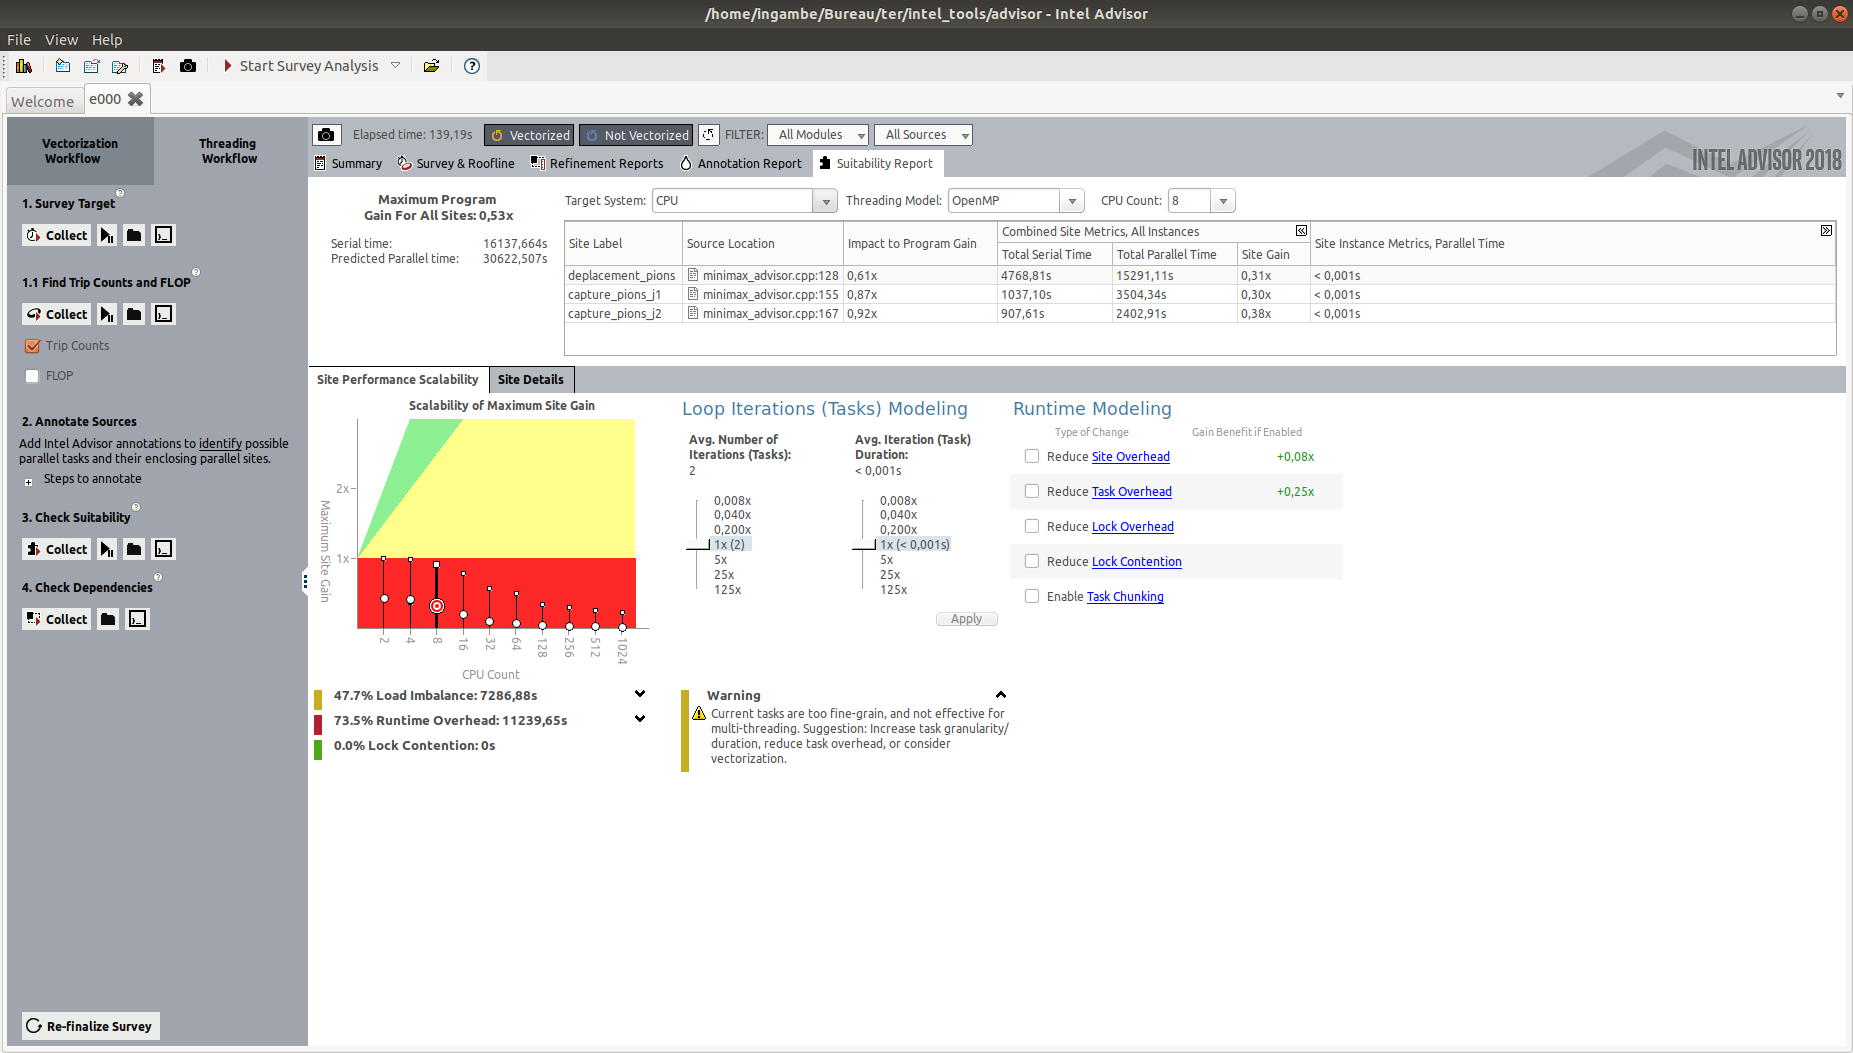
\includegraphics[width=\linewidth, keepaspectratio=true]{suitability.png}
  \caption{Résultat d'Advisor "Suitability"\label{Fig:advisor_suitability}}
\end{figure}

Malheureusement nous pouvons observer que l'ajout de parallélisme à chaque boucle ne fera que ralentir le programme.\\
Le logiciel nous indique que les taches effectués sont d'un granularitée trop fine ce qui induit un "Task Overhead" (le temps passé à créer une tâche et à l'assigner à un thread ainsi qu'à mettre en pause ou arrêter le thread une fois fini) qui est trop important, ce qui pénalise le programme parallèle.\\

\subsubsection{Test de la viabilitée ajout parallélisme}\mbox{}\\

Mal-grès le fait que l'ajout de parallélisme ne soit pas pertinent, nous allons tout de même tester le mode "Dependencies" d'Advisor qui sert à détecter si les hotspots dont l'ajout de parallélisme est pertinent découvert précédemment ne possèdent pas des dépendances de données qui empêchent la parallélisation.\\

\begin{figure}[H]
  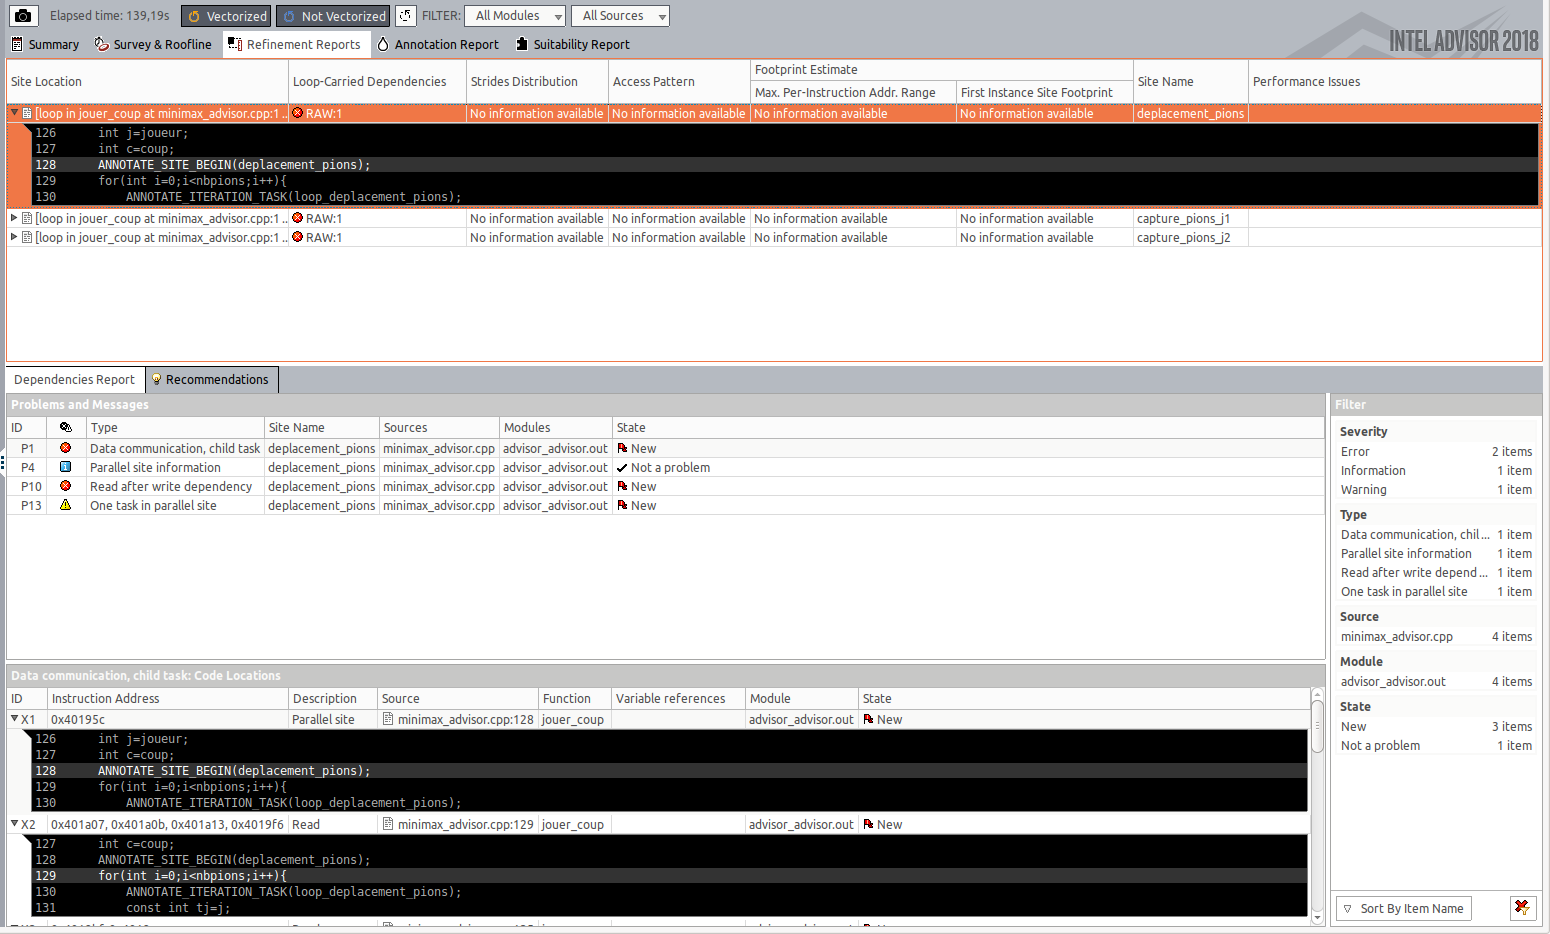
\includegraphics[width=\linewidth, keepaspectratio=true]{dependecies.png}
  \caption{Résultat d'Advisor "Dependencies"\label{Fig:advisor_dependencies}}
\end{figure}

En plus de ne pas être pertinent, l'ajout de parallélisme dans les hotspots n'est pas possible à cause des dépendances de données, Read After Write donc réelles dépendances que l'on ne peut enlever. Et il n'est pas non plus possible d'ajouter du parallélisme dans la fonction decisionAB à cause du fait qu'ils faille remonter alpha et bêta lors de l'évaluation des sous-noeuds afin d'effectuer des coupes.\\ 

\section{Modification algorithmique du code}

Dans cette partie nous allons essayer d'améliorer les performances de notre application en modifiant son algorithme.\\
Ce programme utilise un algorithme de min-max avec coupes alpha bêta, il y a quelques voies d'optimisation possible :
\begin{enumerate}
\item On peut réordonner l'ordre d'évaluation des coups afin de faire jouer les coups statistiquement meilleur en premier (exemple: un puits avec beaucoup de cailloux à plus de chance d'être une meilleur coup qu'un puits avec un unique cailloux). Cela peut améliorer l'efficacité des coupes alpha bêta.
\item On peut créer une table de transposition qui associe une position à un score afin de ne pas avoir a recalculer certaines positions. Vu que l'on doit utiliser une fonction de hachage, il y a potentiellement des collisions qui peuvent changer les coups joués par rapport à la version sans table de transposition, mais il est très facile de tester si tel est le cas.
\item On peut créer un fichier d'ouvertures, avec les X premiers coups pré-calculés à l'avance avec une meilleur profondeur. L'inconvénient de cette solution est qu'elle peut changer les coups joués par la nouvelle version du programme par rapport à la version de base, ce qui empêche la comparaison.
\end{enumerate}

\subsection{Trie des coups à visiter}
Trier à chaque profondeur à un coup trop important, mais trier a la profondeur 0 est pertinent car cela peut aider grandement a améliorer la valeur de alpha et donc de générer plus de coupe dans les sous noeuds, et ce pour un coût négligeable en temps (trie sur les indices d'un tableau de 6 cases).

\subsection{Table de transposition}
On ne peut pas avoir une table de hashage globale car il y a trop de positions possibles à stocker. Cependant, on peut avoir une table de hashage pour le tour courant, qui nous permet de regarder pour chaque noeud, si il a déjà été évalué et cela peut, peut-être nous éviter certains calculs sans pour autant consommer trop de mémoire.

\subsubsection{Ordered Map}
En C++ les std::map sont des arbres binaires de recherche. Pour pouvoir implémenter les maps il faut d'abord changer légèrement la structure de donné contenant la position du plateau, passant d'un tableau deux dimensions à un objet de type std::array à une dimension (ont linéarise simplement le tableau à deux dimensions).

\begin{figure}[H]
  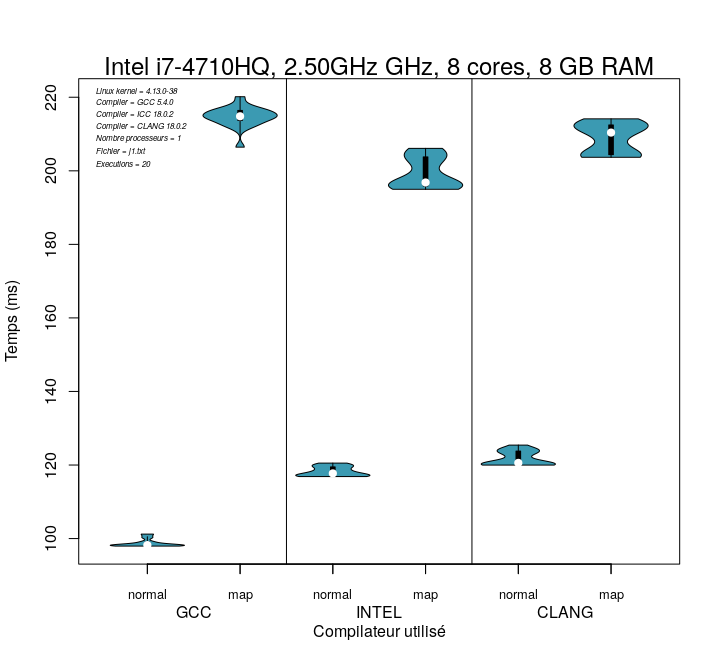
\includegraphics[width=\linewidth, keepaspectratio=true]{sorted_map.png}
  \caption{Ordered Map}
\end{figure}

\subsubsection{Unordered Map}
Nous utilisons une fonction de hachage basique trouvé sur \href{https://stackoverflow.com/a/42701911}{StackOverflow}, c'est une fonction qui comme beaucoup de fonction de hashage est basé sur des xor succesifs. Elle effectue des XOR entre le hash de chacun des éléments du tableau auquel on ajoute un nombre fixe, l'élément décalé de 6 bits vers la gauche et de 2 bit vers la droite.

\begin{figure}[H]
  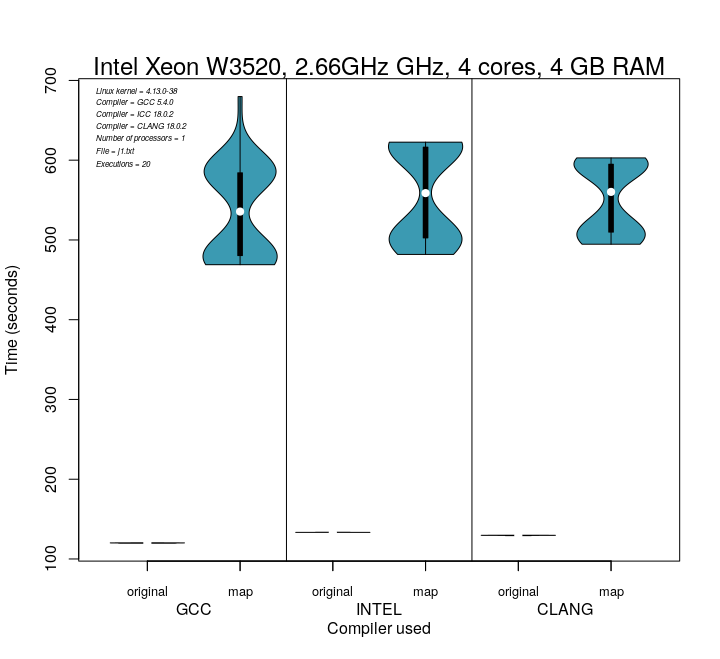
\includegraphics[width=\linewidth, keepaspectratio=true]{unsorted_map.png}
  \caption{Unordered Map}
\end{figure}

Dans les deux cas les performances ne sont pas améliorés, cependant la table de hashage ordonnée donne de meilleurs résultats que la table de hashage non ordonnée, cela semble montrer que la fonction de hashage prend beaucoup de temps à être calculée par rapport au cout de notre fonction d'évaluation (simple différence entre le nombre de cailloux prix par l'ordinateur et l'adversaire).\\
Il est aussi possible que la fonction de hashage ainsi que la structure de donnée ne soit pas optimale pour ce jeux, une possibilitée serait d'implémenter la \href{https://chessprogramming.wikispaces.com/Zobrist+Hashing}{fonction de hashage de Zobrist} et d'utiliser un grand tableau de liste contenant un couple <Hash,Valeur>, pour retrouver la valeur de notre position, il faudrait faire Hash\%TAILLE\_TABLEAU pour obtenir l'indice du tableau et parcourir jusqu'à trouver notre couple <Hash,Valeur>, si le tableau est très grand cela pourrait peut être accélérer le calcul. Cela n'a pas été fait par manque de temps.


\end{document}